
% no longer than 5 pages including figures and tables + as many pages as needed for references
% 2 columns on 8.5 x 11 inch paper
% 10 point Times Roman font on 12 point single spaced leading, 1 inch margins
% 0.25 inch gutter (seeparation between columns)

% Title, author names, affiliations, abstract should appear on first page
% pages should be numbered
% figures and tables should not require magnification, may contain color but should be
% legible in black and white

\documentclass[sigconf,10pt,review,authorversion]{acmart}\settopmatter{printfolios=true,printccs=false,printacmref=false}
\usepackage{geometry}
\geometry{reset, twoside=true, head=13pt,
     paperwidth=8.5in, paperheight=11in,
     includeheadfoot, columnsep=2pc,
     top=57pt, bottom=73pt, inner=72pt, outer=72pt,
     marginparwidth=2pc,heightrounded
     }
\citestyle{acmnumeric}

% REMOVE FOR ACCEPTED
\renewcommand\footnotetextcopyrightpermission[1]{} % removes footnote with conference information in first column
%\pagestyle{plain}

\expandafter\let\csname not=\endcsname\relax
\expandafter\let\csname not<\endcsname\relax
\expandafter\let\csname not>\endcsname\relax

\RequirePackage{pdf14}
\usepackage{unicode-math}

\usepackage{balance}
%% \usepackage{fixltx2e} % travis-ci has an old version of latex and needs this for \textsubscript, etc
\usepackage{mdframed}
%% \usepackage{booktabs}
%% \usepackage{enumitem}
%% \usepackage{amsmath}
%% \usepackage{amsthm}
%% \usepackage{color}
%% \usepackage{calc}
\usepackage{xspace}
%% \usepackage{upgreek}
\usepackage{graphicx}
%% \usepackage{natbib}
%% \usepackage{alltt}
\usepackage{fancyvrb}
%\usepackage{array}
%% \usepackage{tabu}
%% \usepackage{multirow}
\usepackage{mathpartir}
%% \usepackage{balance}
\usepackage{subcaption}
\usepackage{wrapfig}
%% \usepackage{framed}
\usepackage{colortbl}
\usepackage{tikz}
\usetikzlibrary{decorations.markings}
\usetikzlibrary{arrows,shapes}
\usetikzlibrary{positioning}
\tikzset{
    >=stealth,
    %auto,
    %node distance=3.5cm,
    font=\scriptsize,
    ack/.style={align=center,ellipse,draw},%circle,draw,thick,align=center},
    minimum size=20pt
}
\usepackage{multicol}
\usepackage{pgfplots}\pgfplotsset{compat=1.13}


%% Requires:
%% \usepackage{color}
%% \usepackage{calc}
%% \usepackage{xspace}
\usepackage{pifont}

\usepackage{tikz-cd}

%% \usepackage{upgreek}

% \usepackage{MnSymbol}

\setlength{\bibsep}{1pt}

%\newtheorem{theorem}{Theorem}
%\newtheorem{lemma}{Lemma}
%\newtheorem{definition}{Definition}

\definecolor{gray}{rgb}{0.9,0.9,0.9}
\definecolor{red}{rgb}{1,0,0}
\newcommand{\graybox}[1]{\mbox{\setlength{\fboxsep}{0.5pt}%
    \colorbox{gray}{$#1$}}}

%\newcommand{\graybox}[1]{#1}

\newcommand{\var}[1]{\mathit{#1}}

\newcommand{\fixme}[1][\relax]{{\color{red}{FIXME: #1}}}


\newcommand{\ma}[1]{\ensuremath{#1}\xspace}


\title{Four reasons your build is slow}
\author{Sarah Spall}
\affiliation{Indiana University}
\author{Sam Tobin-Hochstadt}
\affiliation{Indiana University}


\begin{abstract}
Spending time waiting for code to compile is cliche enough to be
featured in XKCD, yet it continues to plague software
developers. Fortunately, software builds are an embarassingly parallel
problem, and so we can finally make use of all those extra cores---a
happy coincidence of software complexity and hardware trends.
%
Unfortunately, the story is not quite this rosy, as almost anyone who
waits for software to build knows. Real build systems fail to be the
embarassingly parallel poster child we hope for, and instead are slow
in a wide variety of ways.

To investigate this problem, we have built an automated build analysis
tool that works for arbitrary build systems using the venerable
\texttt{make} tool. Our analysis can predict parallel speedup, analyze
the long pole of dependencies, determine false dependencies, and
predict parallelism in a perfect world. We use our tool on real-world
project to describe four problems found in actual software builds, and
in some cases how to fix them.
\end{abstract}


\begin{document}

\maketitle

\section{Introduction}

If you develop software, or even if you compile it, you probably run
into software that's slow to build. This problem is such a cliche that
it appears in comics, but it's also such a problem that companies
routinely outfit developers with the beefiest machines possible---all
to compile software projects faster. Fortunately, for most systems and
languages, compiling software is a classic example of embarassing
parallelism. As a result, developers who spend much of their time
compiling large software projects use highly parallel systems to do so
\cite{regehr-tweet}.

This is perhaps best demonstrated by the classic \verb|make -j|
command, which builds on \verb|make|~\cite{make} to execute
dependencies in parallel, consuming as many parallel resources as are
available. The process-oriented nature of \verb|make| and the graph
structure of dependencies combine for easy and effective parallelism.

However, this seeming solution rarely works out as well in practice as
it does in theory. In addition to the substantial expense of
highly-parallel systems, real software rarely makes use of the full
capacity of the machine despite the potential for high
degrees of parallelism.

To address this problem, numerous new build systems have been created
(Bazel, Buck, Pants, Aegis, Shake, CMake, Ninja, ...), many purporting
to solve or at least alleviate these problems. However, systems
software ranging from the Linux kernel to LLVM to zlib is still built
with \verb|make| today, suggesting that as in many areas, building new
tools is not sufficient---we must analyze, understand, and improve use
of existing tools as well.

To accomplish this for build systems, we have developed a tool for
analyzing \verb|make|-based builds by instrumenting them while they
run, relying on \verb|make|'s own internal information and the use of
\verb|strace| to analyze the behavior of the actual commands used to
run the build. Our tool computes a dependence graph based on the
actual behavior of the build, then prunes it with data from
\verb|strace|. The resulting graph can accurately predict the
potential parallelism of the build from the instrumentation, show what
build steps cause the biggest slowdown, and answer counterfactual
questions about the results of improving the build system.

After describing our analysis tool, we present four case studies in
reasons software might be slow to build, backed by data and analysis
from our tool. All of the case studies are real, widely-used
open-source projects. In some cases, we identify low-hanging fruit
that can increase the parallelism of a build by 4x; in others we point
to places where code organization changes could make a significant
difference. These case studies demonstrate the benefits of a
build-system analysis tool and point to valuable further investigation.



\section{Analysis tool}
\label{sec:analysis}
In this section we describe the tools we use to analyse make builds, diagnose problems related
to parallelism, and identify places for improvement. In section \ref{sec:makeanalysis} we
discuss the modified version of GNU Make \cite{gnumakemanual} we use to record enough information about a
project's build to reconstruct the build graph during a post-mortem analysis.
In section \ref{sec:straceinstr} we discuss how we use a slightly modified version of strace to
record all of the system calls made during the project's build and then use the system calls
to determine the real dependencies of the build. In section \ref{sec:revisegraphs} we discuss
how to combine the information from these two tools to transform a build graph into
a new graph with potentially more parallelism.

\subsection{Make analysis and instrumentation}
\label{sec:makeanalysis}

To collect the desired level of information from a run of GNU Make \cite{gnumakemanual}, we run it with the
debug level of 'verbose', use our own wrappers, which print additional information, and use
a modified version of make which prints directory and timing information for each shell command run.
All of this information is written to a file and later used to reconstruct
the build graph of a successful build.  The reconstructed graph contains all of the shell commands
executed during the build as well as the time each one took to complete.  With the structure of the
build and the timing information the work and span of the build can be calculated. Work is the total
time to execute every shell command in the build graph, and span is the longest time to execute any
sequence of shell commands which must execute sequentially.  For example, the span of a single
make rule is, the longest time to execute a dependency plus the sum of the times to execute each
recipe.  Parallelism is defined as \begin{math} \frac{span}{work} \end{math}, therefore to increase
the parallelism of a project the span must be decreased; making span an important place to focus
performance improvements.

Identifying the span path in a build identifies the most important places for performance
improvements.  In section \ref{sec:realanalyses} we discuss four causes of parallelism
performance issues in make based project builds, how to use this tool to identify the
issue and use information about the span of the build to implement a solution.

% Have a wrapper around gnu make; which prints information about which top-level make
% is being invocated and prints out the directory; this wrapper also times the call to
% actual gnu make

% have a 2nd wrapper around gnu make; which is called for ``sub makes''. we tell actual
% make that we want it to call this for all $(MAKE) calls in the makefile.  this wrapper
% similarly to the top-make wrapper prints out which make is being executed as well as the
% directory and time of the actual make call.
% WHY do we need the above information??

% The most important change is in make itself; where we modified make to print each shell
% command it is running as well as the time the shell command took.
% this data lets us calculate the work and the span of the build and lets us attribute span
% to the correct targets and shell commands.
% Since we are able to store the command run by make in the reconstructed build graph we can
% rerun those ocmmands to replay the build; and it didn't require us to parse the makefile
% ourselves.

% tool can calculate work and span of the build and attribute the span to the correct nodes
% so that the user can focus their performance improvements on the portiosn of the graph that
% will have the most affect.

\subsection{Strace instrumentation}
\label{sec:straceinstr}

To extend the analysis performable on build graphs, strace \cite{strace4.25} is used in
conjunction with our enhanced version of GNU Make.  Strace can capture and record the system
calls of every process launched during a make build, allowing us to later map directly between
a shell command launched by make and the system calls it ran.  Strace can write the system call
information for each pid used to its own file.  This is a good way to map directly from a
shell command to a set of system calls, except that Linux may reuse pids during the course of
a build, which causes strace, by default, overwrite these files.  To solve this problem and
maintain a 1 to 1 mapping between processes launched by make and system call information,
we modified strace to append a timestamp to each file extension along with the pid.

When the system call data is mapped to a command, the data is processed to determine which
files were inputs and which files were outputs of that command.  An input file could have been
read by the command but not written, and an output file could have been written by the command.
Whether or not a file is an input or output depends on which system calls refer to the file.
Using this information the build graph can potentially be modified and we discuss this more
in the next section.

% strace lets us capture and record the system calls of every process launched during a make build
% and it will save each process pid's system calls to an individual file which makes it easy for
% us to map each shell command to its system calls.  There is one wrinkle in this plan though,
% pids can be reused and pid reuse is not strictly increasing and the version of strace that we
% used would overwrite a file if this occured which results in inaccurate data. 

% to solve this problem we have strace also append a timestamp to the end of the output file
% extensions.  This results in unique output files which are also strictly increasing with
% respect to the timestamps.

% we then parse the strace information to determine which files were touched by a process and
% we classify these files as input files and as output files.  Two processes which only share
% input files should in theory be able to run in parallel.  So using this information we can
% modify the make graph to allow those two processes to run in parallel. 

\subsection{Revising graphs}
\label{sec:revisegraphs}

A build graph is made up of two types of vertices and two types of directed edges.  A vertex is
either a leaf, representing a file or a shell command executed by make, or a non-leaf,
representing a target.  An edge is either a dependency edge, or a recipe edge.
Dependency edges leaving the same vertex may run in parallel with one another, but must all
complete before any recipes edges leaving the vertex may be run.  Recipe edges leaving the same
vertex must run sequentially in a predetermined order after all dependency edges have been run.

To increase the span of a build graph recipe edges need to transform into dependency
edges if possible.  To determine if it is possible system call data is used to calculate the
file inputs and file outputs of each shell command.  If two adjacent recipes share zero or more
input files and share no input and output files, then those two commands can run in parallel.

For each vertex in the original graph, the inputs and outputs are calculated for each
dependency and recipe.  And an \emph{input-output} graph is built using this information.  If two
recipes intersect in more than just their inputs, there is an edge from the recipe that executes
first to the recipe that executes later.  Every recipe is compared to every other recipe and to
the set of dependencies to build this \emph{input-output} graph.  The recipes that can be safely
run in parallel are determined by calculating the lowest level of the graph each vertex is at.
Recipes may run in parallel with other recipes or dependencies at the same level, but must run
after all recipes and dependencies at lower levels have completed.  After the new graph is
constructed the same analysis that was performed on the original graph can be performed on the
new graph.  Whether or not the new graph has a lower span is dependent upon whether or not
transformed edges fall within the original span path or not.

% build graph is made up of two types of node and two types of edges.  A node is either a
% leaf node which represents a file or represents a single shell command executed by make, and
% a non-leaf node which represents a single target.  And an edge is either a dependency edge or
% a recipe edge.  A dependency edge points to another node which must be run before recipe
% edges of the node may be run.  All dependnecy edges may be run in parallel while the recipe
% edges must be run sequentially, so there is an explicit ordering on recipe edges.

% To increase the parallelism of a build graph we want to transform recipe edges into
% dependency edges if possible.

% to do this we combine the build graph we constructed with the strace data we collected to
% compare the input and output files of each recipe run as well as each command.  If two
% adjacent 

\section{Make build analyses}
\label{sec:realanalyses}

In this section we discuss four problems with project builds that use make.  In section \ref{sec:expensive},
we discuss
builds whose spans are dominated by a single expensive command that prevents the build from
achieving greater parallelism, look at a project that exhibits this behavior, and explain our
our tool can diagnose this problem and identify areas for improvement.  In section \ref{sec:sequential}
, we discuss what
it means for a build to be unnecessarily sequential, and look at an example of a build that
exhibits this behavior, and how our tool can diagnose this problem and identify areas for improvement.
In section \ref{sec:scalability}, we discuss when a build should have ample available parallelism
but fails to achieve that
parallelism in practice, look at a project that exhibits this behavior, and discuss potential causes.
In section \ref{sec:compiler} we discuss another instance of an expensive command dominating a
build's span; in this case a
slow compiler, we look at a project that exhibits this behavior and how our tool can diagnose it
and identify areas for improvement.

\subsection{Expensive command}
\label{sec:expensive}

\begin{figure}[t]
  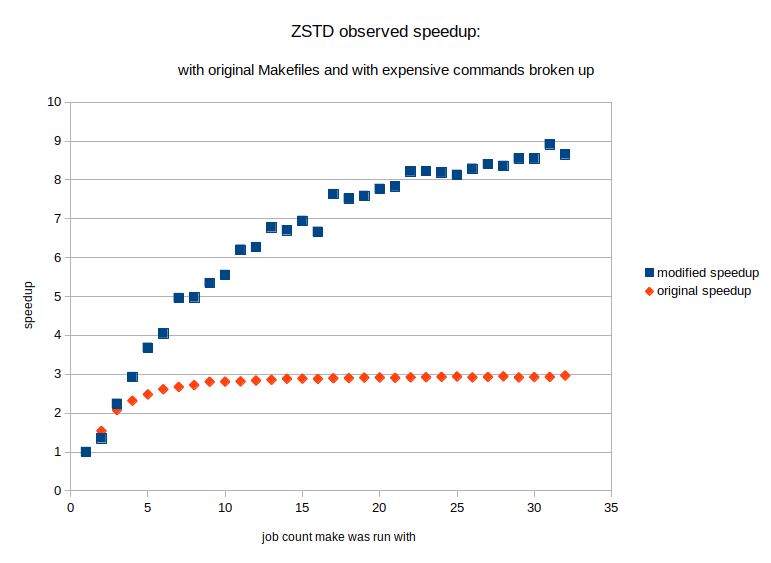
\includegraphics[width=0.5\textwidth]{zstd-speedup}
  \caption{Speedup of zstd's original build when built with regular make,
    compared to speedup of zstd's modified build described in section \ref{sec:expensive}
  when built with regular make.}
  \label{fig:zstd}
\end{figure}

All project builds which lack the desired parallelism can be characterized as having too great of
a span in relation to their work.  The span in a build system is the longest (in time) series of
tasks that must be executed sequentially.  In some cases the span is not a series of similar length
tasks, but is dominated by a single long running task.  In cases like these it is best to identify
the most expensive task in the span, because reducing the running time of that task is the
most likely way to make progress towards increasing the parallelism of the build.

To diagnose the problem of a span dominated by a single long running task, our tool can be used
to learn the span path through the build graph and learn which target and shell commands
are the most time intensive.  To see what sort of an improvement would occur in the span if the
running time of the most expensive target in the span was to decrease, the tool will recalculate
the span of the graph excluding its most expensive member any number of times.  This is useful
in the case where decreasing the running time of a single task gives the build graph a new span
path with a similarly long running time, which is dominated by a different long running command.

Facebook's zstd project \cite{zstd1.3.7} has a build that exhibits this property.  When we used our tool to analyse
the span of zstd's build we saw that it is dominated by a single call to cc; see fig. \ref{code:cc1}.

\begin{figure}[H]
\begin{Verbatim}[commandchars=\\\{\},codes={\catcode`$=3\catcode`^=7\catcode`_=8},fontsize=\small,numbers=left,xleftmargin=5mm]
  cc \$(FLAGS)
  ../lib/common/debug.c
  \textrm{\emph{26 more .c files}}
  zstdcli.o fileio.o bench.o
  datagen.o dibio.o -o zstd
\end{Verbatim}
\caption{A long running cc command which was responsible for about 97\% of zstd's span.  It compiled and linked 27 .c files.}
\label{code:cc1}
\end{figure}

If this call is no longer part of the span, the new span is similarly dominated by another single call to cc;
see fig. \ref{code:cc2}.
\begin{figure}[H]
\begin{Verbatim}[commandchars=\\\{\},codes={\catcode`$=3\catcode`^=7\catcode`_=8},fontsize=\small,numbers=left,xleftmargin=5mm]
  cc \$(FLAGS)
  common/debug.c
  \textrm{\emph{29 more .c files}}
  -Wl,-soname=libzstd.so.1 -o libzstd.so.1.3.7
\end{Verbatim}
\caption{A long running cc command which was responsible for aproximately 100\% of zstd's span when \ref{code:cc1} was not a membe rof the span.
This command compiled and linked 30 files.}
\label{code:cc2}
\end{figure}
If neither of these calls are members of the build's span, then our tool predicts the span would be
approximately 7.2 seconds rather than 39 seconds, as with the original span, or 37 seconds, as with the second span.
This is about an 80\% reduction in the build's span, and the parallelism improves from 2.98 to 16.

To test this we manually replaced the cc command in fig. \ref{code:cc1} with the code in fig.
\ref{code:cc3}.  The original command is replace by a new target for each object file and target
that can build each object file in parallel and link them together afterwards.

\begin{figure}[H]
\begin{Verbatim}[commandchars=\\\{\},codes={\catcode`$=3\catcode`^=7\catcode`_=8},fontsize=\small,numbers=left,xleftmargin=5mm]
../lib/common/debug.o: ../lib/common/debug.c                                                       
    cc \$(FLAGS) ../lib/common/debug.c
\textrm{\emph{26 more targets; one for each object file}}    
zstd-build: \$(OBJ\_FILES)
    cc \$(FLAGS) \$(OBJ\_FILES) -o zstd
\end{Verbatim}
\caption{Makefile targets which replaced original code in fig. \ref{code:cc1}}
\label{code:cc3}
\end{figure}

Similarly, the code in fig. \ref{code:cc2} is replaced by the code in fig. \ref{code:cc4}.  Once
again each object file is explicitly declared as its own target and a target is declared that can
build these object files in parallel and then link them together afterwards.

\begin{figure}[H]
  \begin{Verbatim}[commandchars=\\\{\},codes={\catcode`$=3\catcode`^=7\catcode`_=8},fontsize=\small,numbers=left,xleftmargin=5mm]
common/debug.o1: common/debug.c
    cc \$(FLAGS) common/debug.c
       -o common/debug.o1
\textrm{\emph{29 more targets; one for each object file}}
libzstd-build: \$(OBJ\_FILES)
    cc \$(FLAGS) \$(OBJ\_FILES) -shared
       -o libzstd.so.1.3.7
\end{Verbatim}
\caption{Makefile targets which replaced original code in fig. \ref{code:cc2}}
\label{code:cc4}
\end{figure}

Figure \ref{fig:zstd} shows that when the modified build was run with 1 to 32 jobs,
the predicted speedup was observed.  An additional performance improvement that was not predicted
is that the work of the new build decreased from approximately 120 seconds to approximately 80 seconds.
This is because each of the object files is declared as its own target, so make can consider whether
or not the file already exists and if it is necessary to rebuild it.  In this case, it turns out that
the object files being built as part of the cc command in fig. \ref{code:cc1} had already been built
by make; making it unnecessary to build them again.  This cuts the effect time of the code in fig.
\ref{code:cc1} from about 40 seconds to about 2 seconds; just the time to link the object files.

\subsection{Unnecessarily sequential}
\label{sec:sequential}

Makefiles are a collection of rules which describe how to build targets \cite{gnumakemanual},
and each rule consists
of a a series of prerequisites and a series of recipes which are run to build the target.  The
prerequisites can be built in parallel, but the recipes must be run in the order they are listed.  So,
the author of a makefile can directly impact the potential parallelism of the build by
how they organize their makefile.  It is possible to unnecessarily list things as recipes that
could have run in parallel.  Here we will look at an example of this and how our tool can
discover that these recipes don't actually need to run in parallel.

In the previous section we discussed zstd's build, which turned out to be unnecessarily sequential
because two single shell calls which compiled and linked many files at once could be broken up
into many parallel compilation jobs which could then be linked after.  These two commands could
have been written as follows, respectively, instead of as they were
originally in fig. \ref{code:cc1} and fig. \ref{code:cc2}, and would have resulted in the same
build performance, but would make it possible for our tool to detect that they are unnecessarily
sequential.

The following code is an alternative to the code in fig. \ref{code:cc1}. Each file is compiled individually
as its own recipe, followed by a recipe to link the object files together.  This has the same
performance as the original command.
  \begin{Verbatim}[commandchars=\\\{\},codes={\catcode`$=3\catcode`^=7\catcode`_=8},fontsize=\small,numbers=left,xleftmargin=5mm]
cc \$(FLAGS) ../lib/common/debug.c
   -o ../lib/common/debug.o
\textrm{\emph{26 more recipes; one for each .c file that needs to be compiled}}
cc \$(FLAGS) \$(OBJ\_FILES) -o zstd
\end{Verbatim}
  
The following code is an alternative to the code in fig. \ref{code:cc2}. Each file is compiled individually
  as its own recipe, followed by a recipe to link the object files together.  This has the same
  performance as the original command.
  \begin{Verbatim}[commandchars=\\\{\},codes={\catcode`$=3\catcode`^=7\catcode`_=8},fontsize=\small,numbers=left,xleftmargin=5mm]
cc \$(FLAGS) common/debug.c -o common/debug.o1
\textrm{\emph{29 more recipes; one for each .c file that needs to be compiled}}
cc \$(FLAGS) \$(OBJ\_FILES) -shared
   -o libzstd.so.1.3.7
\end{Verbatim}

  These recipes compiling individual files can run in parallel, as shown in the previous section,
  and our tool can detect this by using the build graph and the system call information gathered
  by strace and applying the methods described in section \ref{sec:revisegraphs}.  When the span
  of the new graph is calculated it reflects the fact that these compilations can occur in
  parallel and is 8 seconds rather than the original 45 seconds; these times are longer than
  those mentioned in the previous section because strace inflates the running time of the
  commands it traces.

\subsection{Bad scalability}
\label{sec:scalability}

\begin{figure}[t]
  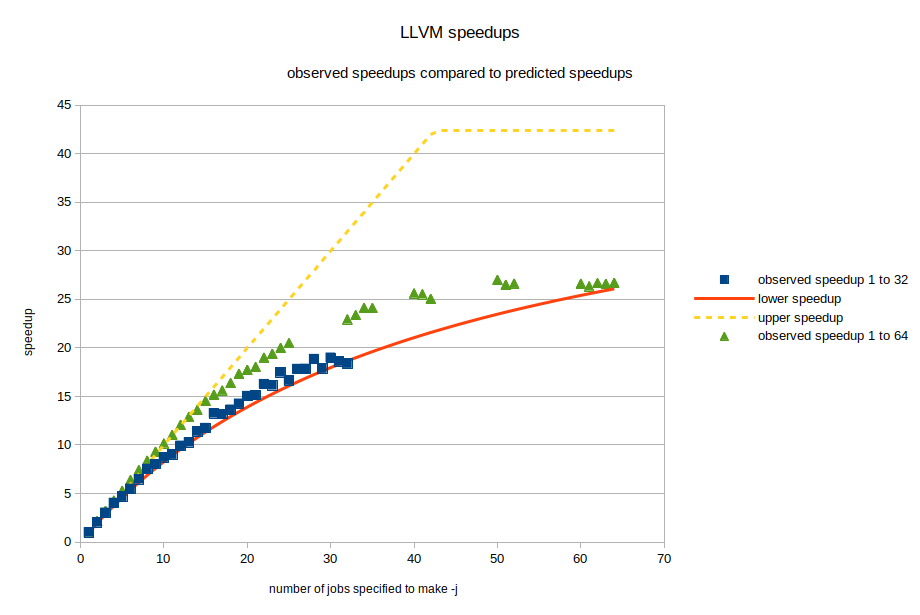
\includegraphics[width=0.5\textwidth]{llvm-speedup-w-64}
  \caption{A comparison of the observed speedup when LLVM was built with \emph{make -j <n> for <n> from 1 to 32},
    to the potential speedups our tool predicted using the work and span calculations}
  \label{fig:llvm}
\end{figure}

Some projects may exhibit ample potential parallelism but may not achieve that potential
parallelism in practice.  LLVM~\citep{LLVM:CGO04} is the largest
project we analysed, with a calculated work of approximately 12584 seconds, or 3.5 hours.
With a predicted span of 305 seconds, or 5 minutes, LLVM has a parallelism of about 41.
These calculations where made from a build of LLVM that was run without strace.

A parallelism of 41 lead us to believe that when built in parallel on a machine with 32 cores,
LLVM should build in about 5 minutes.  Our observations did not match this expectation.  When LLVM was
built with ``-j 32'' the observed speedup was slightly over 18; see chart~\ref{fig:llvm}.  Using work and
span our tool can predict the potential speedup a build will experience using Brent's theorem
\cite{brents}.  The lower speedup bound is predicted using Brent's theorem, which specifies that for
P processors, \begin{math} T_P \leq T \end{math}

% say something about brent's theorem
% say something about why llvm doesnt achieve the predicted speedup

% project example is LLVM:
% say something about how LLVM is a very large project and 

\subsection{Slow compiler}
\label{sec:compiler}

An issue similar to the one described in section \ref{sec:expensive} is a build's
span being dominated by the compilation of a single file.  This problem cannot be
solved in the makefile like the issue in section \ref{sec:expensive} was.
Possible solutions to this problem include
breaking the file up into smaller files which can be compiled in parallel and then
linked, or changing the compiler so it is capable of compiling the file faster.
A faster compiler would likely have the additional benefit of not only decreasing the span
of the project but also likely decreasing the work of the project.

Google's protocol buffers project \cite{protobufs3.6.1} exhibited this behavior.  It's work was calculated
to be about 16.7 minutes and it had a relatively
long predicted span of 43.7 seconds, which was dominated by a call to g++ compiling
a single file.  When the analysis applied in section \ref{sec:expensive} is applied
to protocol buffers' build, we learn that the top three spans are dominated by the
single file compilations of the files in fig. \ref{code:g++1}.  If the g++ compilations
of these three files were not in the build's span the new span would be about 20s,
roughly half of the original span.  Speeding up the compilation of these three files
would be a good place to begin improving the parallelism of this build.

\begin{figure}[H]
\begin{Verbatim}[commandchars=\\\{\},codes={\catcode`$=3\catcode`^=7\catcode`_=8},fontsize=\small,numbers=left,xleftmargin=5mm]
  google/protobuf/descriptor.cc
  google/protobuf/descriptor.pb.cc
  google/protobuf/compiler/cpp/cpp\_message.cc
\end{Verbatim}
\caption{The compilation of these 3 files dominate the longest 3 spans.}
\label{code:g++1}
\end{figure}

% so, if the problem is with compiling a single file, then we don't really have a
% make level solution to that problem
% user needs to do some work at the file/compiler level to create a solution
% potential solutions include breaking the file up into smaller files which can be
% compiled and linked in paralle
% using a faster compiler, which would have the added benefit of likely decreasing
% the overall work of the build as well as the span
% maybe trying to motivate some future work here

% example project is protobufs c++ version;
% We perform the same analysis that we did in section expensive;
% look at the top spans and what they are dominated by
% we see that the top 3? are dominated by g++ compilations of single files
% and if those are no longer part of the span we half our span; which would result in a
% double speedup
% so we now have a place to focus our energy for improvements
% HIgh level; non make level fix; expensive section is a make level fix; should mention that
% there maybe

\section{Conclusion}

We present an automated analysis tool for build systems based on
\verb|make|, which can automatically determine the available
parallelism in a build process and provide useful information to
improve it. Our tool makes use of \verb|strace| instrumentation to
determine the ground truth about the build process, and can answer
counterfactual questions about how much a build could improve.
%
We show four case studies on three real software projects
demonstrating the power of our analysis and point to sources of
slowdown and lack of parallelism, and use our tool to make
improvements that substantially increase parallelism.

The case studies we've shown already demonstrate the value of our
tool, but extensions could make it more useful to developers and build
system authors---for example, by automatically generating revised
\verb|Makefile|s or by using \verb|strace| to instrument arbitrary
build systems, not just \verb|make|. Finally, we hope to integrate
this with an analysis of parallelism in commands executed by the build
system, such as the \verb|gold| linker.

\bibliographystyle{ACM-Reference-Format} 
\bibliography{citations}
\balance

\end{document}
